\chapter{Methods}
\label{chapter:methods}

This chapter describes the research methodology used to examine the success of the design described in the previous chapter. The research setting, process and data analysis methodology are presented. 

The design in chapter \ref{chapter:design} involves many choices which may have affected the performance of the robot as a sign language tutor. Resources were not available to validate all of those choices. The interaction scheme of the robot was chosen as a likely candidate to influence tutoring effectiveness, and so the following study was designed. This study also serves as an example of how the design framework can be used more broadly: fixing other design parameters, and varying one to measure its effect of success.

Three different interaction schemes of the robot, referred to here as design conditions, were compared. The study of the robot's and the child's interaction was framed as a comparative design study. The research question relevant for this chapter is RQ2: Is the designed robot successful as an assistive sign tutor? This was examined by testing three hypotheses: 


\vspace{3mm}

\noindent\textbf{H1: Children will imitate signs performed by the robot}
\vspace{3mm}

\noindent\textbf{H2: The design condition will affect the success of imitation}
\vspace{3mm}

\noindent\textbf{H3: The design condition will affect the child's attention focus}
\vspace{3mm}

These hypotheses, and how they were tested, is discussed further in this chapter.


\section{Research setting and process}

Experiments with 12 autistic children were organized to examine their responses to the robot InMoov as an assistive sign tutor. The experiments were organized at Satakunta's hospital district, in collaboration with speech therapist Lehtonen and neuropsychologist Nyman. A script for the robot to follow during the experiments was created together with the speech therapist. The experiments lasted around 30 minutes per child, with the speech therapist and a companion of the child (parent or other care-taker) present with the child in the experimentation room. The robot was operated from the next room by myself and another engineer, according to instructions given by the speech therapist via a camera feed. The therapy session was observed by the operators through three camera feeds. After the therapy session, the child and their companion were asked to fill out short surveys to describe their experience. The surveys along with footage from the camera feeds were analyzed after the experiments, using both quantitative and qualitative methods.


\subsection{The InMoov and its modifications}

The InMoov is a human-sized humanoid robot torso, controlled by Arduino microcontrollers, constructed out of 3D printed plastic body components and gears. The power is distributed through custom printed circuit boards, also available under the CC BY-NC license. The fully assembled robot has 29 servo motors controlled by two Mega Arduino boards. A USB hub connects the Arduino boards and peripherals (in our case a mouth speaker and an eye camera) to the controlling computer, which in this case was a Windows laptop. The software used to control the robot, MyRobotLab, is an open source robot control framework \cite{inmoov}. 

\begin{figure}
\centering
  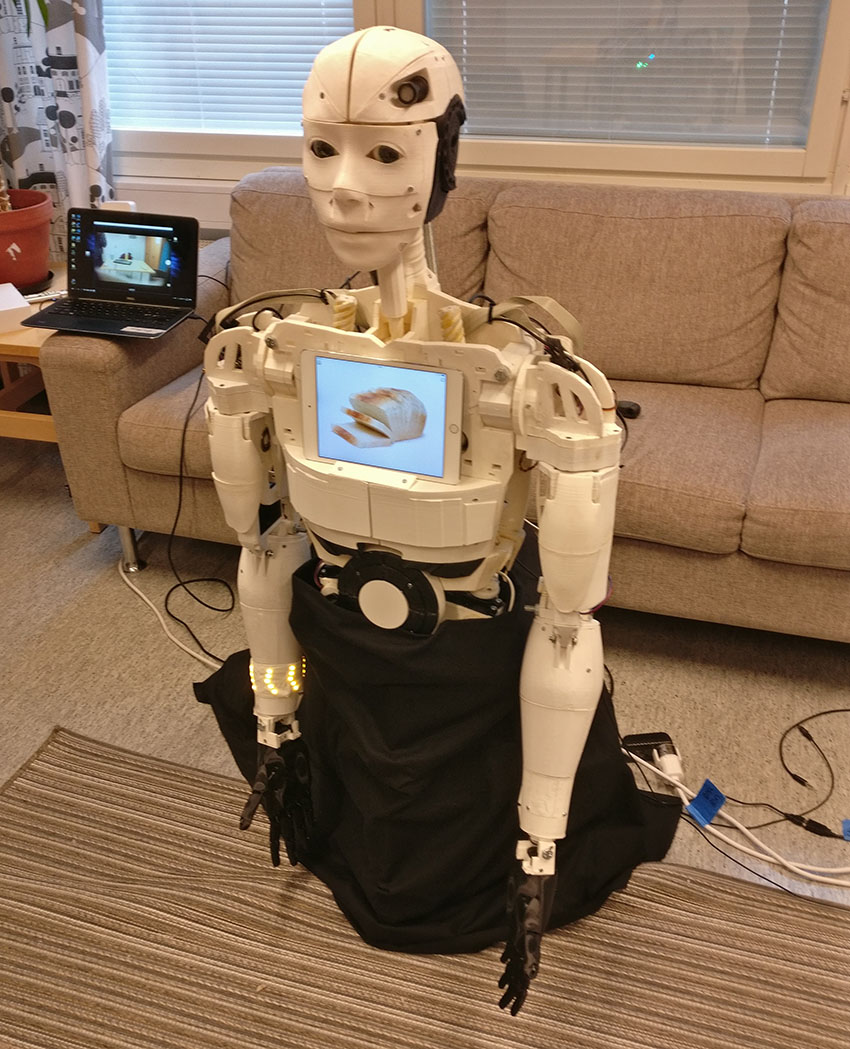
\includegraphics[width=8cm]{images/momo_on_floor.jpg}
  \caption{The robot pictured in the experimentation room, with both the lights on the hand and the picture on the tablet active.}
  \label{fig:momo}
\end{figure}

The implementation of the InMoov used in this experiment can be seen in figure \ref{fig:momo}. The InMoov used in this experiment was built using the original schematics, and printed out of ABS and PLA plastic, with additional NinjaFlex in the hands. Its original hands were replaced by Ada hands, the schematics for which are also available online under a Creative Commons license CC-BY-SA \cite{adaOpenbionics}. The original hands are visible in figure \ref{fig:inmoovhands}, while the new hands are visible in figure \ref{fig:adahands}. The signs were performed solely with the robot's arms and hands. The InMoov had 2 degrees of freedom (DOF) in each finger, including its thumb. Its wrists had 2 DOF, biceps 4 DOF, and shoulders 4 DOF. The InMoov was powered by an adjustable bench power supply with 6 V. The Ada hands were powered through two 12 V AC adapters.

\begin{figure}
\centering
  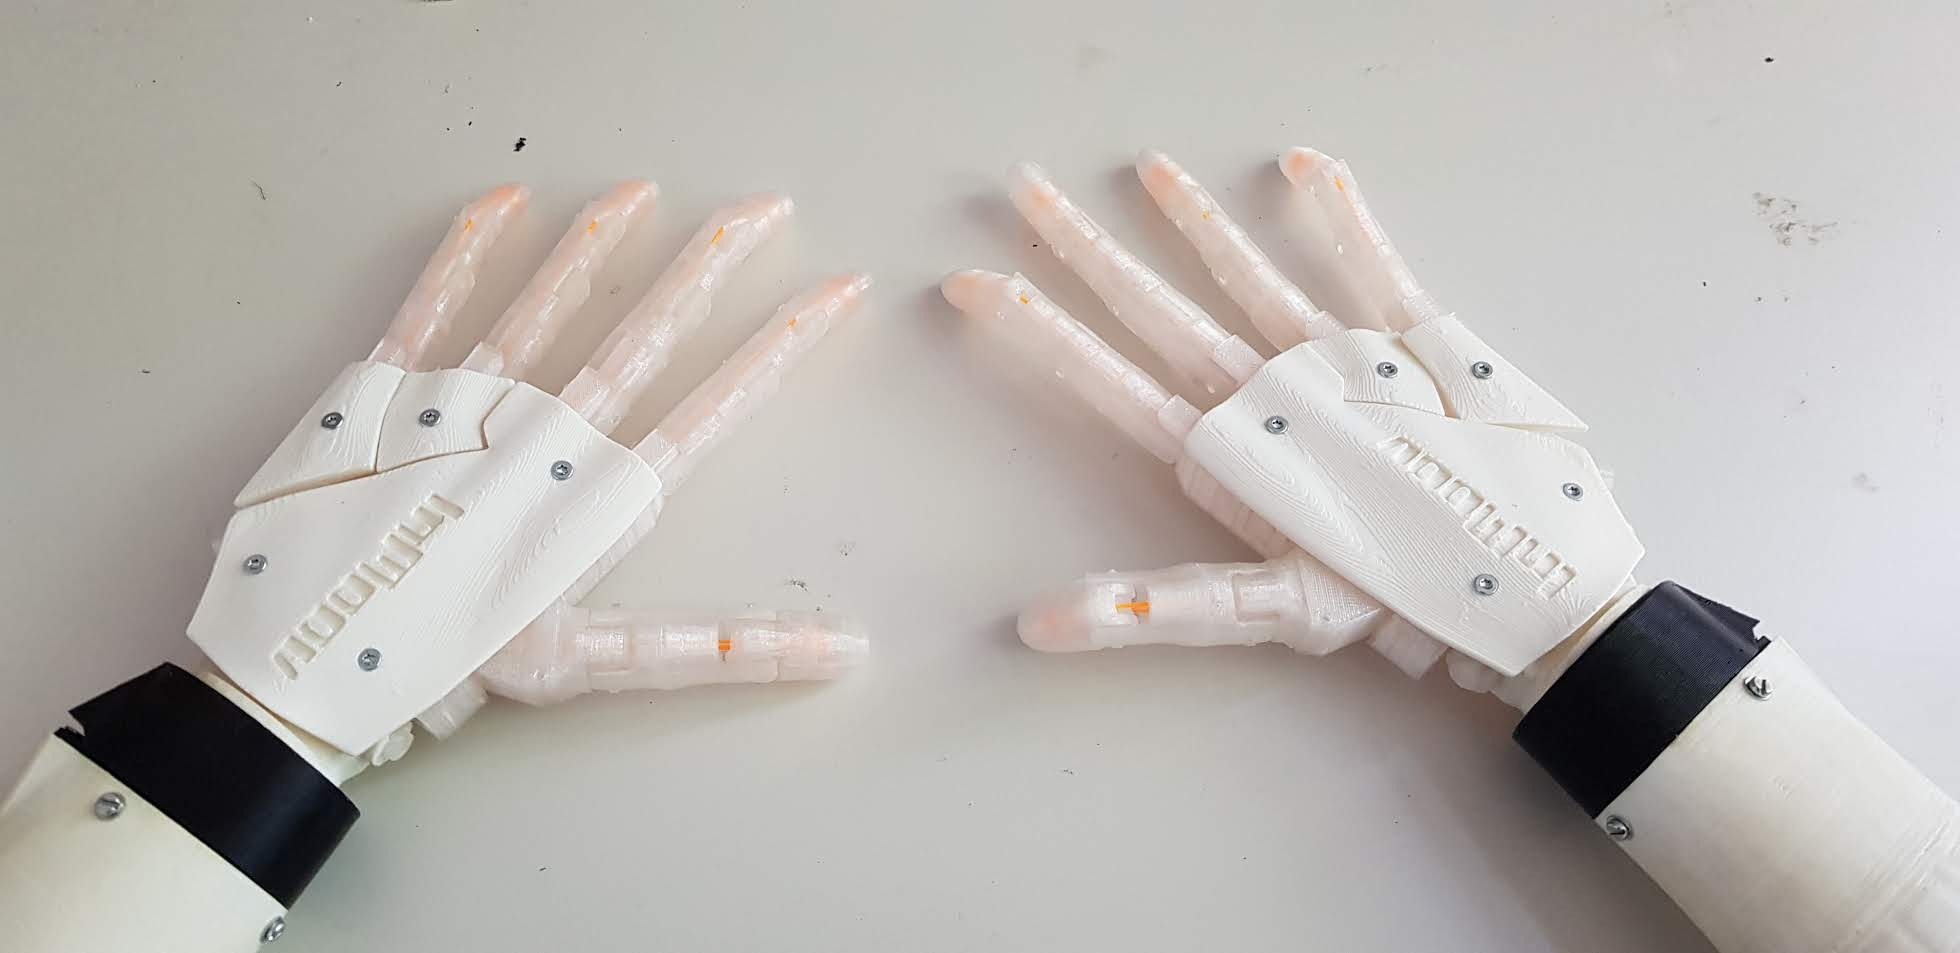
\includegraphics[width=\linewidth]{images/Inmoov-hands.jpg}
  \caption{The InMoov's original hands.}
  \label{fig:inmoovhands}
\end{figure}

\begin{figure}
\centering
  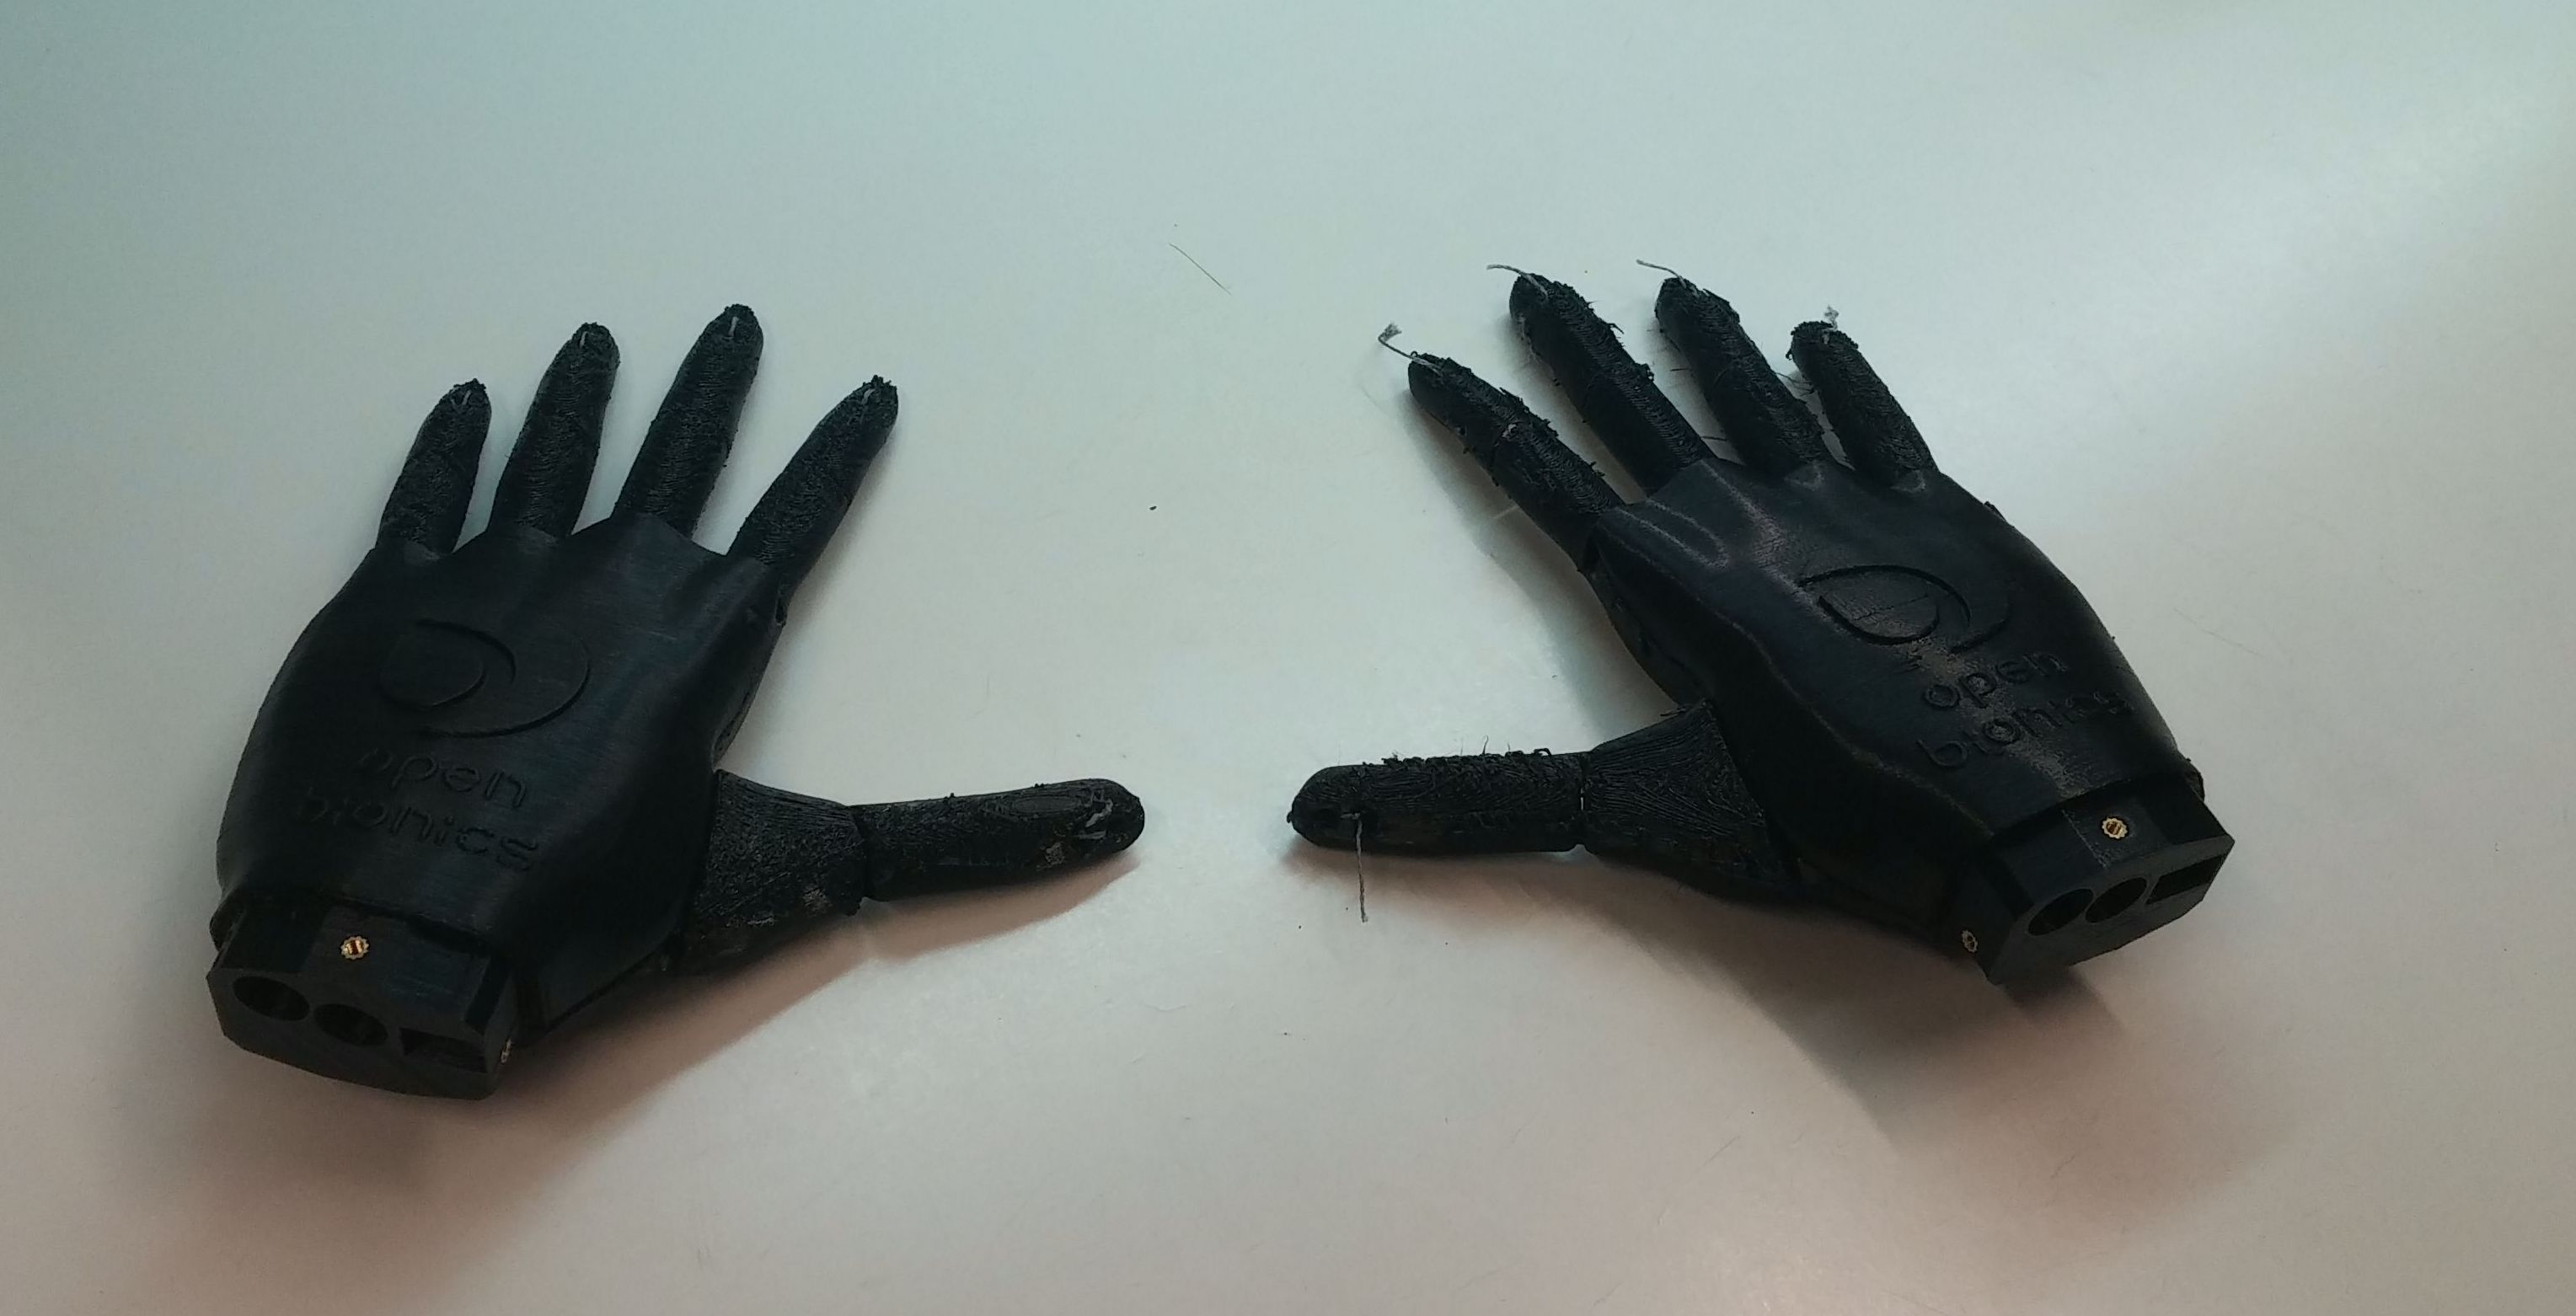
\includegraphics[width=\linewidth]{images/Ada-hands.jpeg}
  \caption{The new Ada hands.}
  \label{fig:adahands}
\end{figure}

The InMoov's chest components were modified to fit a tablet screen, and lights were attached to its right hand with tape. To control the robot during the experiments, commands were executed through MyRobotLab. Unique command sequences were written for each child, which were executed according to what the operators observed to be happening in the experiment room. The tablet in the robot's chest was also controlled through MyRobotLab.


\subsection{Signing with the InMoov}

9 signs were selected for the experiment together with the speech therapist. The signs are depicted in figures \ref{fig:viittomat1} and \ref{fig:viittomat2}. The thumbs up gesture that the robot performs during the experiments is also depicted in figure \ref{fig:viittomat2}. When choosing these signs, the physical limitations of the InMoov were taken into account: the InMoov is unable to cross its arms over its midsection, could not raise its shoulders, and could not bend its wrists. All of the signs were non-abstract concepts, such as animals or sports, which children were familiar with beforehand. These signs would be taught in assistive signing therapy even without the robot. Before the signs were used in the experiments, the speech therapist verified the recognizability of the signs with a colleague who did not know the set of signs. This procedure was adapted from the sign language study performed with Robovie R3 \cite{uluer2015new}.


\begin{figure}
\centering
  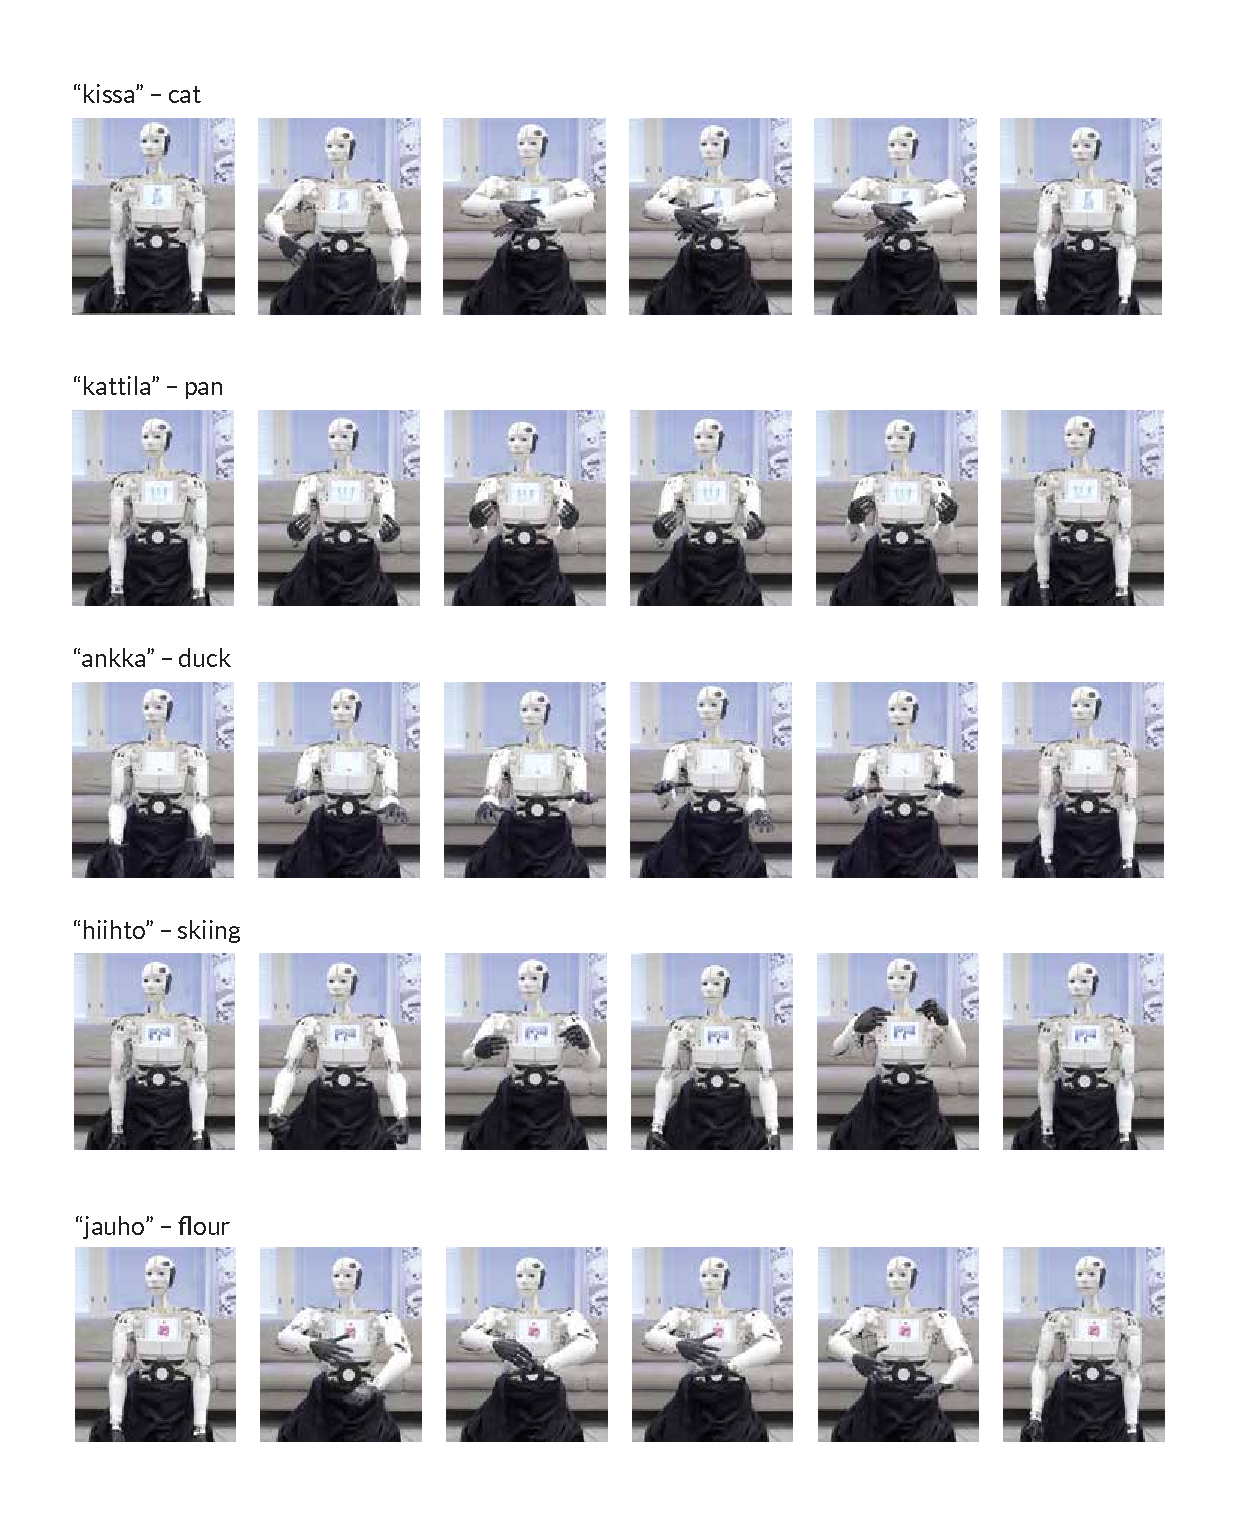
\includegraphics[width=\linewidth]{images/viittomat1.pdf}
  \caption{Five signs out of the set of nine.}
  \label{fig:viittomat1}
\end{figure}

\begin{figure}
\centering
  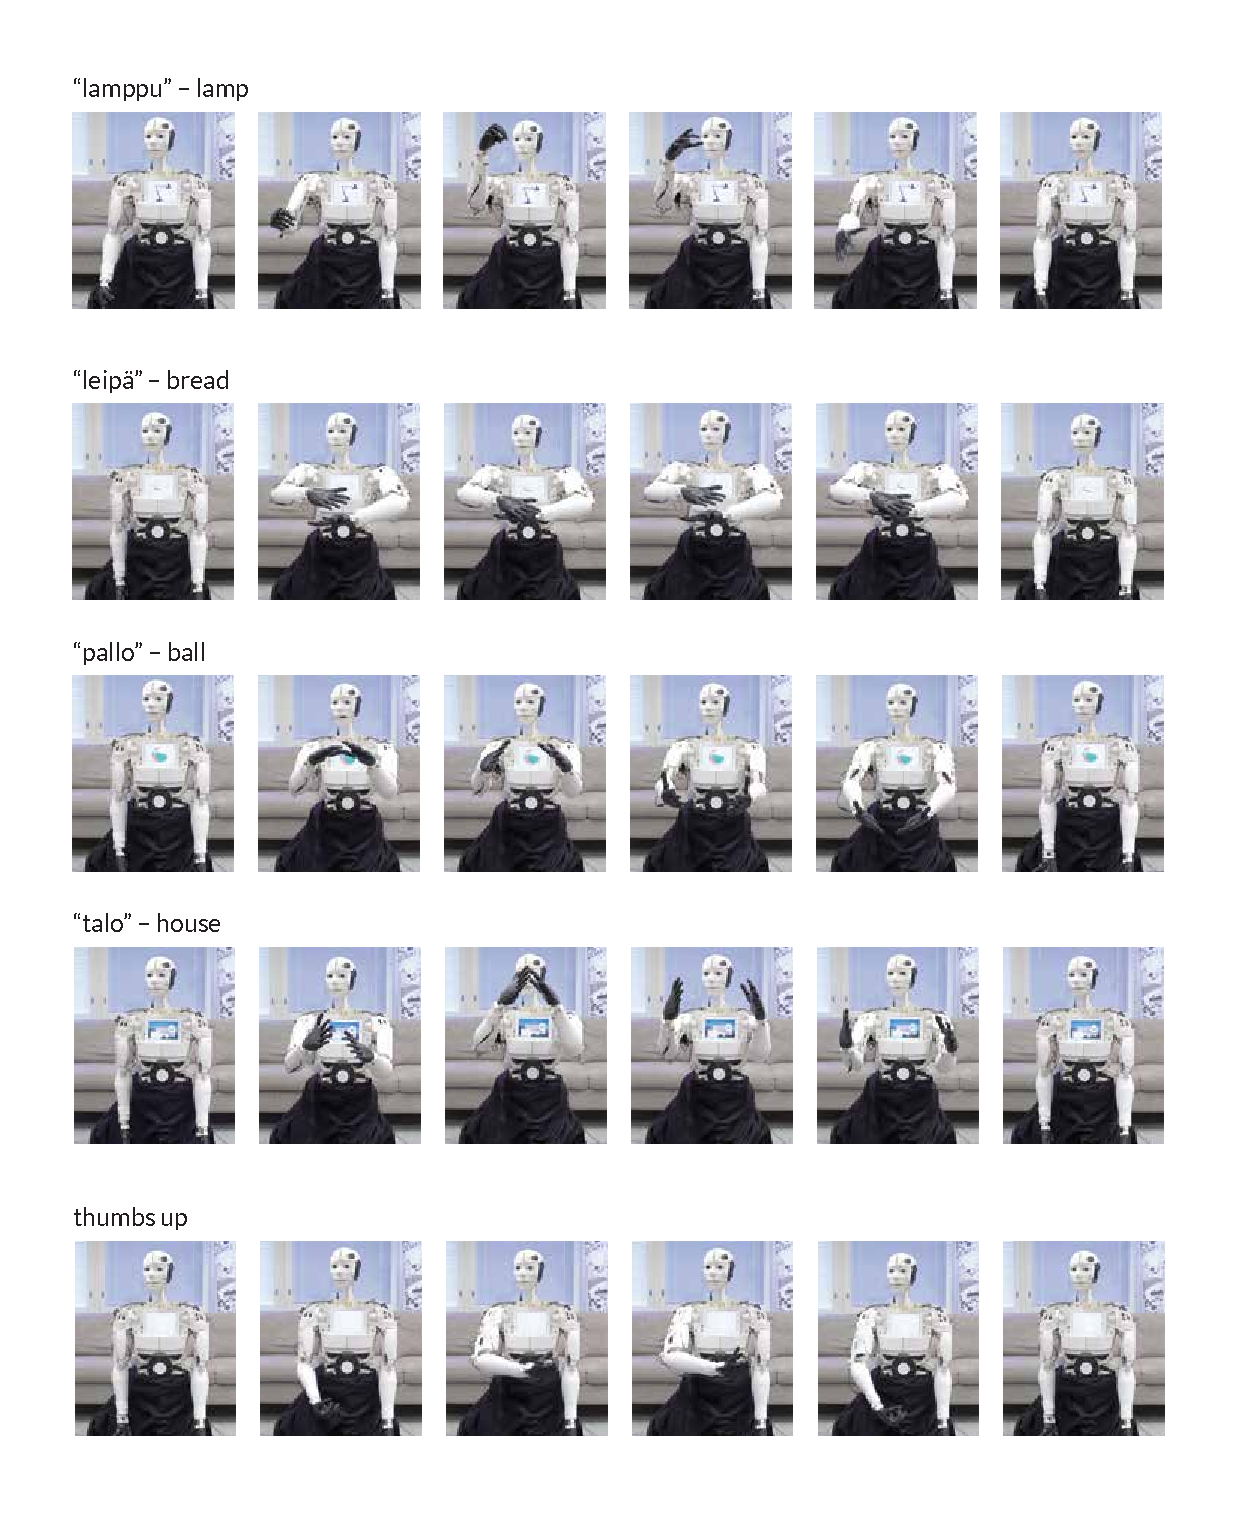
\includegraphics[width=\linewidth]{images/viittomat2.pdf}
  \caption{Four signs out of the set of nine, and the thumbs up gesture that the robot makes to reward the child.}
  \label{fig:viittomat2}
\end{figure}


\subsection{Research participants}

10 out of the 12 children that took part in the experiments were analyzed. Two of the experiments had to be discarded from data analysis, one due to a mistake in the operation of the robot, and the other after the child's parent stopped the experiment since the child could not calm down. The participants' ages, severity of autism and companions in the experiment are detailed in table \ref{table:participants}.


\vspace{0.5cm}
\bgroup
\def\arraystretch{1.3}
\begin{table}
\centering
\begin{tabular}{ c | c | r }
  \textbf{Age} & \textbf{Autism severity} & \textbf{Accompanying person(s)}\\
  \hline
  13 & mild & mother \\
  23 & severe & caretaker \\
  14 & severe & caretaker \\
  13 & severe & mother \\
  14 & mild & mother \\
  11 & severe & mother \\
  16 & severe & caretaker and psychologist \\
  14 & severe & two caretakers \\
  11 & mild & mother and father \\
  16 & severe & two caretakers \\
\end{tabular}
\vspace{0.5cm}
\caption{A list of the experiment participants' ages, autism severity, and accompanying persons.}
\label{table:participants}
\end{table}
\egroup


\subsection{Experiment set-up}

The experiment was set up in a room at the facilities of Satakunta's hospital district, in collaboration with speech therapist Lehtonen and neuropsychologist Nyman. The experiment set-up is seen in figure \ref{fig:roomSetup}. The experimentation room was familiar to some of the children beforehand. Some of the children came from home, and some lived at the hospital's quarters. All children were accompanied by either a parent or a caretaker from the hospital.

\begin{figure}
  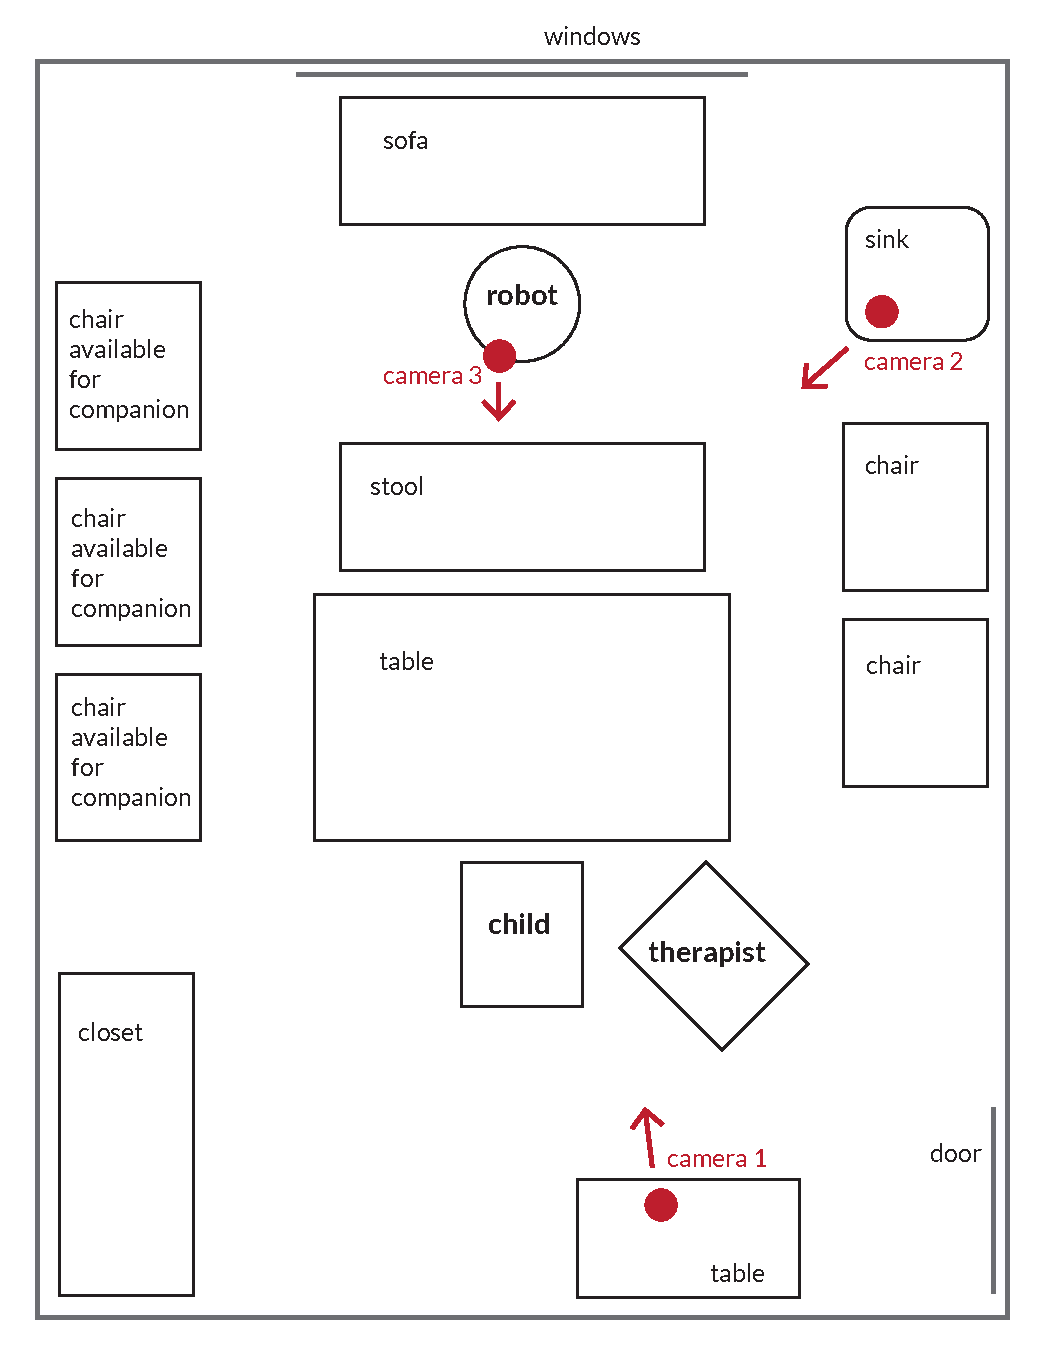
\includegraphics[width=\linewidth]{images/room_setup.pdf}
  \caption{The experiment set-up. The child sat directly in front of the robot, with a table in between them, for the safety of the child. The speech therapist sat next to the child, facing the child and the robot. Three cameras were placed in the room, in order to capture all of the child's behavior. The child's companion could choose one of the three seats on the side of the room.}
  \label{fig:roomSetup}
\end{figure}

The robot was at the back of the room on the floor. The child was sat at a table directly facing the robot. The speech therapist sat diagonally next to the child. The companion of the child sat in one of the chairs along the sides of the room, wherever they felt most comfortable.

The table was placed between the user and the robot to discourage physical contact in order to ensure physical safety of the child, and of the robot, as the robot is fragile. Some of the test users were also known to display aggressive behavior on occasion, so the table acted as a protector of both the robot and the child.

The robot was teleoperated from a room across the hall. An observer observed the experiment room through three camera feeds, and told the operator which functions to execute, according to the speech therapist's signals. The speech therapist indicated to the operator that the child signed correctly, incorrectly, or that the child had not responded as all. Cameras were placed behind the child, to the front of the child, and in the robot's right eye. The view front the front camera can be seen in figure \ref{fig:front}, and the back camera in figure \ref{fig:back}. In accordance to the ethics consideration defined in the design process, the footage recorded by the cameras that was used to generate data was treated with care, and kept encrypted.

\begin{figure}
\centering
  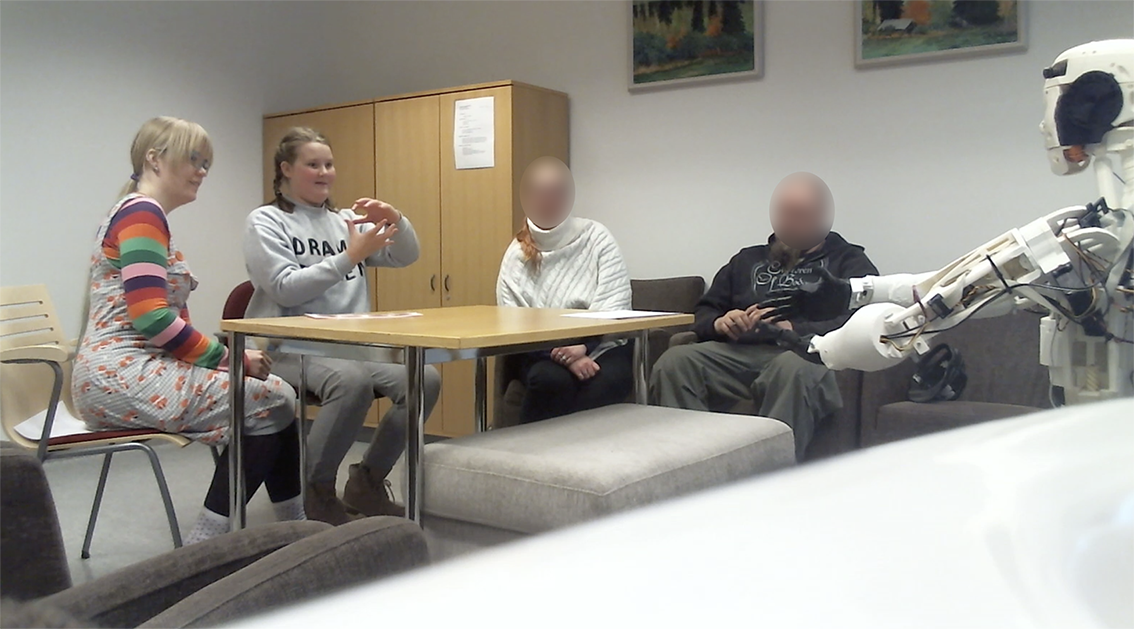
\includegraphics[width=\linewidth]{images/experiment_front.png}
  \caption{View from the front camera, with the robot signing ``flour".}
  \label{fig:front}
\end{figure}

\begin{figure}
\centering
  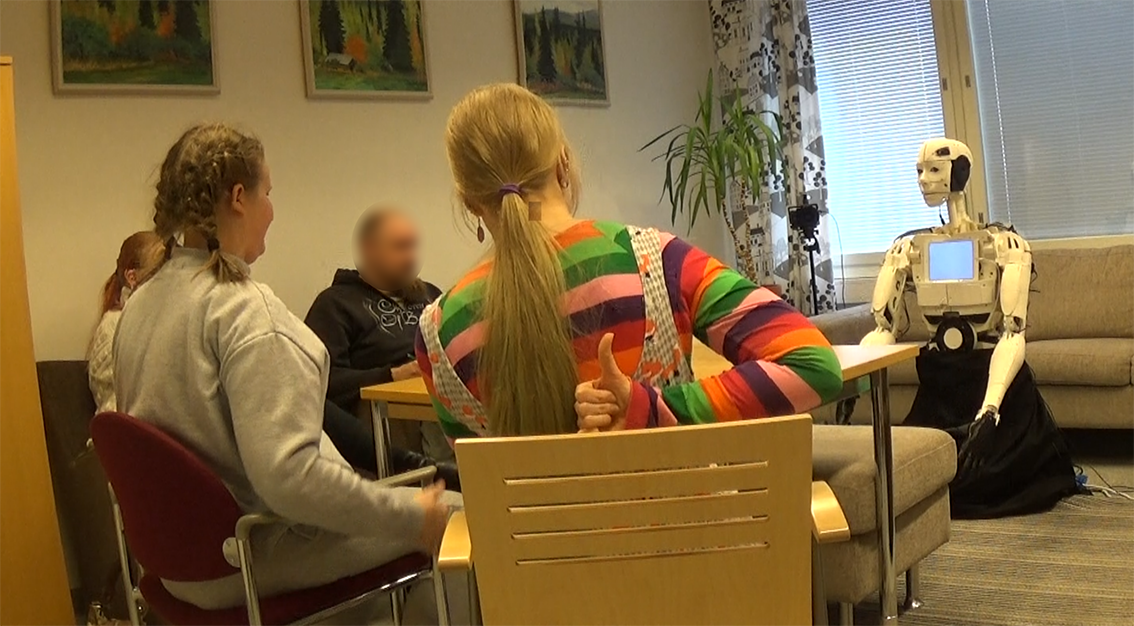
\includegraphics[width=\linewidth]{images/experiment_back.png}
  \caption{View from the back camera, with the speech therapist showing to the camera that the child had signed accurately.}
  \label{fig:back}
\end{figure}


\subsection{Experimental procedure}

The experimental procedure was precisely defined beforehand, as was discussed in the previous chapter.

When the child first entered the experimentation room, the speech therapist showed the child a picture series of how the experiment would proceed. This procedure was adapted from the study done with the robot Tito and children with autism \cite{duquette2008exploring}. The picture series is visible in appendix \ref{chapter:explanation}. This was done to create some familiarity with the robot so the child could feel more comfortable \cite{duquette2008exploring}, and to help the child know what to expect. After the experiment ended, the child and their companion were asked to give their opinions via surveys. The child's survey is visible in appendix \ref{chapter:children}, and the companion's survey is visible in appendix \ref{chapter:companions}. The survey was administered by neuropsychologist Nyman, who entered the experiment room after the interaction with the robot had concluded. After completion of the surveys, the child and their companion promptly left the experimentation room.

For the experiments themselves, an interaction structure was programmed beforehand for each child. The programmed interaction structure included each child's name, and a randomized order for the signs. For each sign, one of three different design conditions was randomized. Three signs were assigned randomly to each condition. The design conditions were made up of different interaction modalities. The design conditions were:

\begin{itemize}
  \item Sign and voice command
  \item Sign and voice command, and image in chest tablet
  \item Sign and voice command, and flashing lights in right hand
\end{itemize}

The image condition can be seen in figure \ref{fig:momo}, and the images shown on the tablet are seen in figure \ref{fig:tabletimages}. The image always corresponded with the word being signed. The lights on the robot's hand can be seen in figures \ref{fig:lights} and \ref{fig:momo}. The lights were turned on when the robot started signing, and switched off when it stopped signing.

\begin{figure}
\centering
  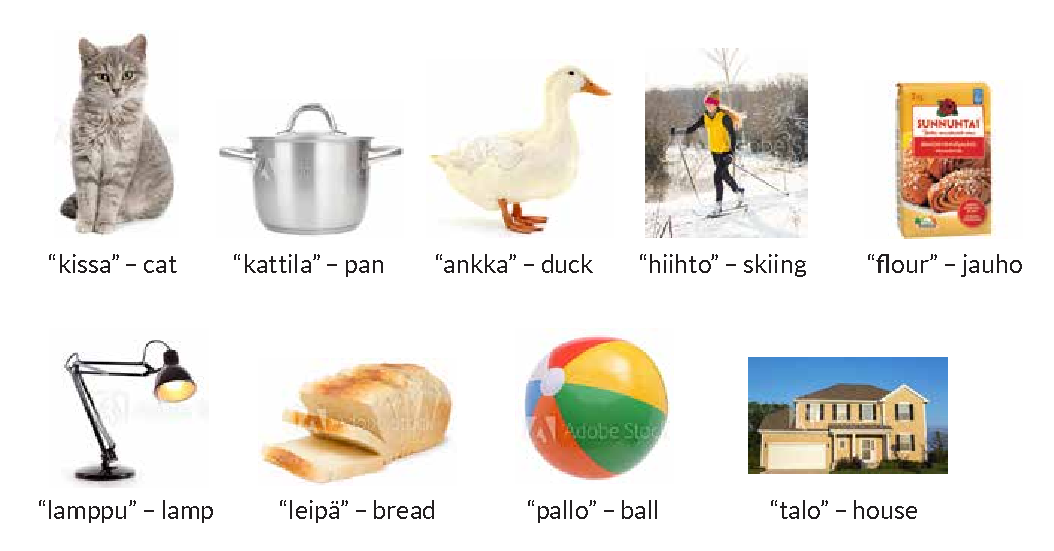
\includegraphics[width=\linewidth]{images/tablet_images.pdf}
  \caption{Images shown on the tablet simultaneously with the word spoken in the second design condition.}
  \label{fig:tabletimages}
\end{figure}

\begin{figure}
\centering
  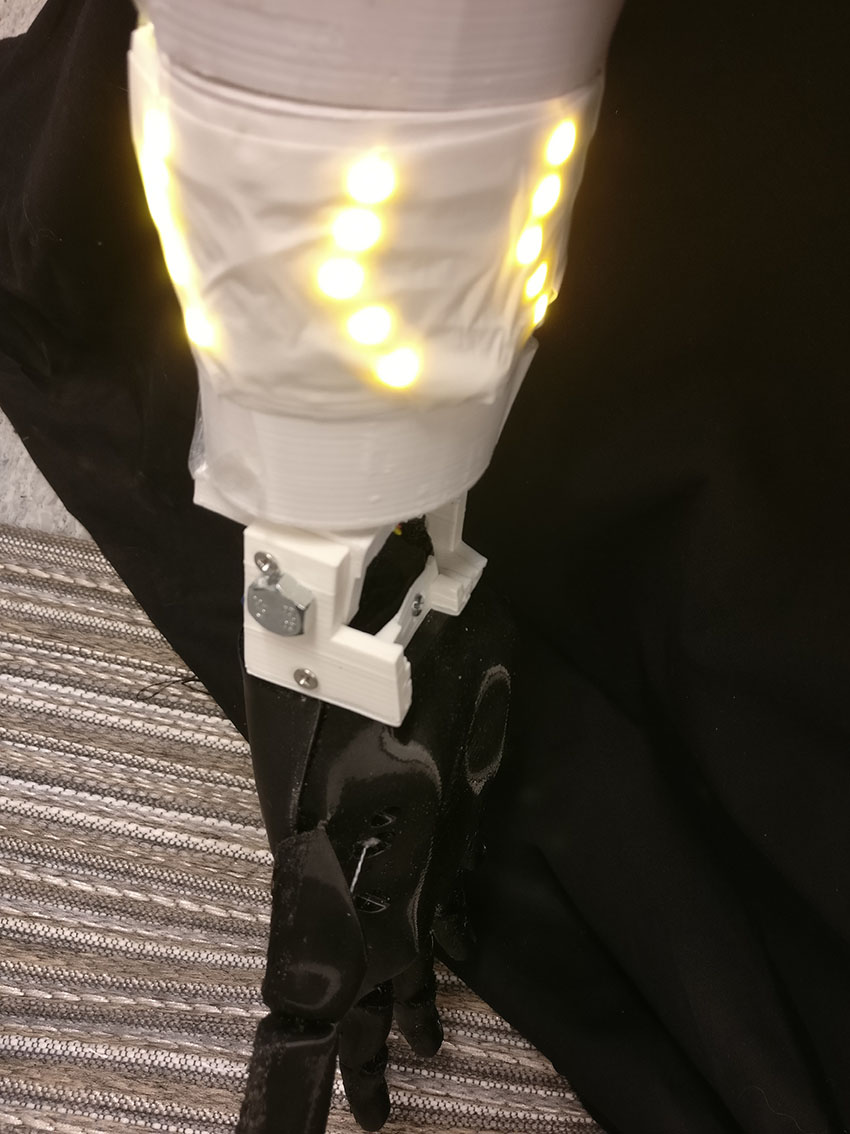
\includegraphics[width=4cm]{images/lights.jpg}
  \caption{The lights attached to the robot's hand for the third design condition.}
  \label{fig:lights}
\end{figure}

The basic interaction structure used during the experiments is depicted in figure \ref{fig:flowchart}. The robot demonstrated a sign, asked the child to respond, and then responded appropriately to the child's response. The robot demonstrated nine signs overall during each experiment. At the start of the experiment the robot said hello, and at the end of the experiment the robot said goodbye. A more detailed conversation transcript is attached in appendix \ref{chapter:conversation} in Finnish.

\begin{figure}
\centering
  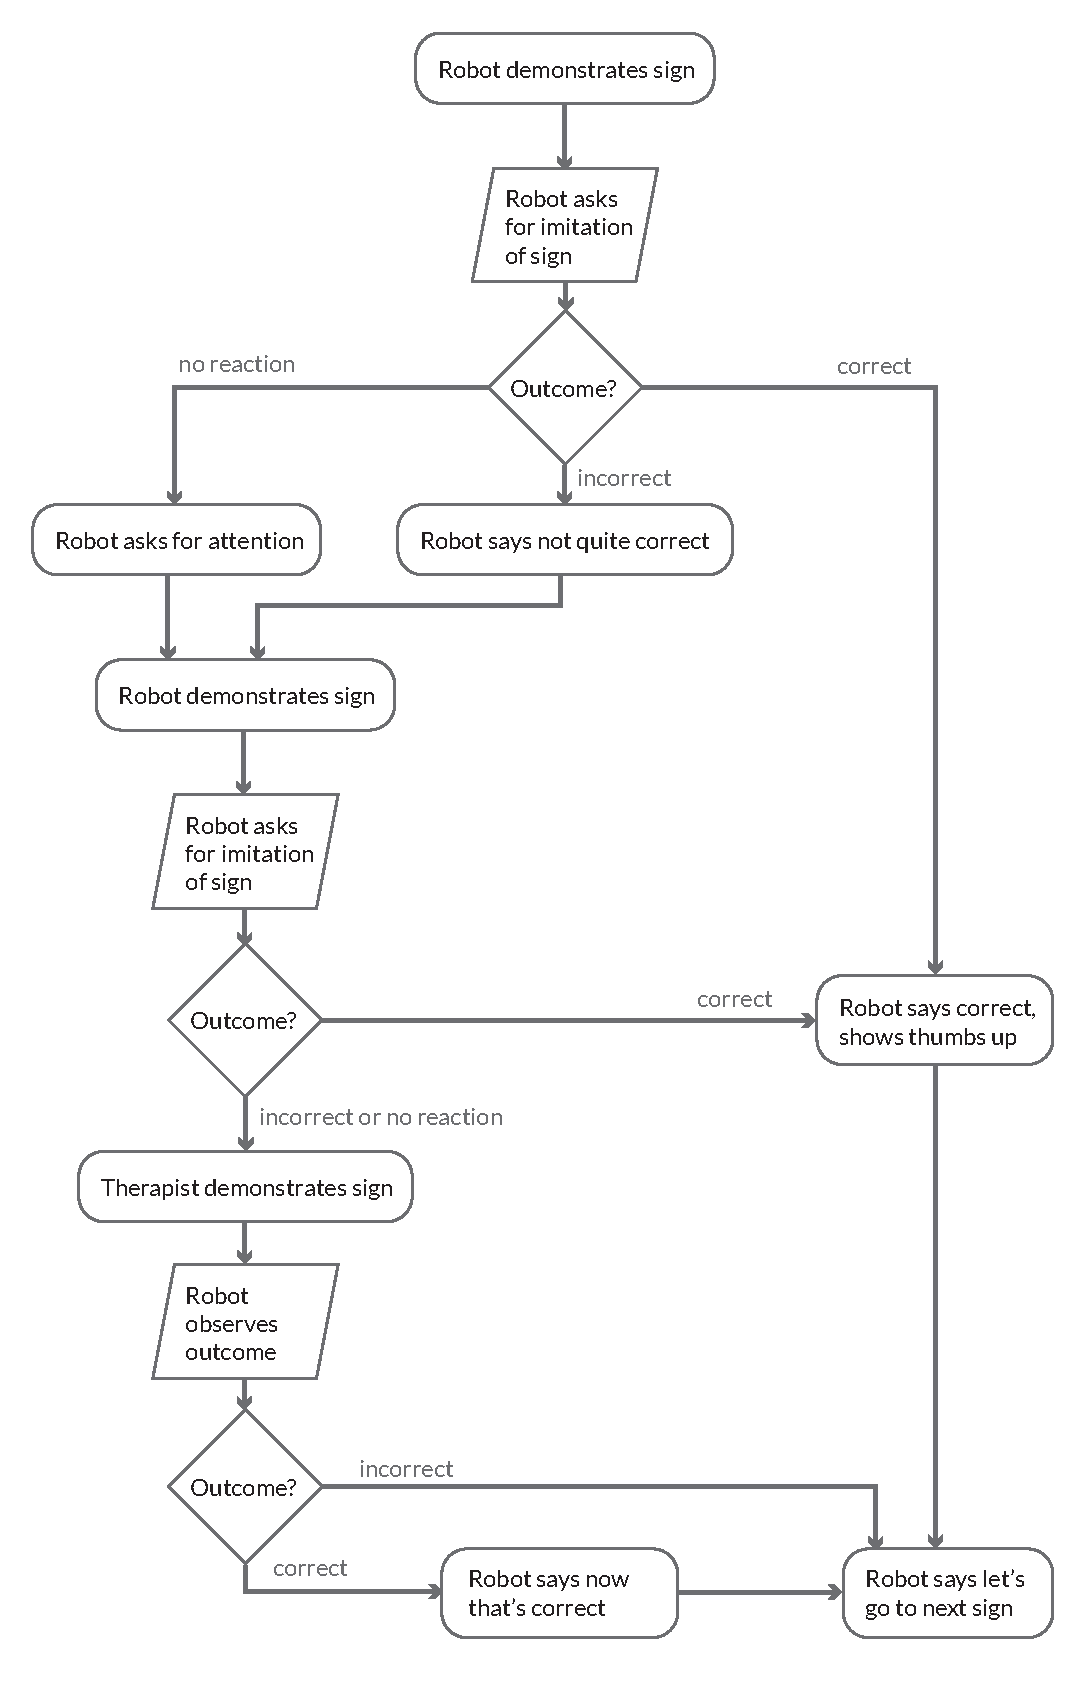
\includegraphics[width=\linewidth]{images/behavior_flowchart.pdf}
  \caption{Flowchart of the robot's behavior, which was executed by the operators according to the child's responses.}
  \label{fig:flowchart}
\end{figure}

%%%%%%%%%%
%%%%%%%%%%


\section{Research methodology}

The primary research methodology was examining and analyzing the videos of each child interacting with the robot. Due to the small amount of quantitative data anticipated to be gathered from the videos, it was triangulated with qualitative data gathered from the surveys conducted with the children and their companion after the experiment.

H1, H2 and H3 were tested primarily through the video data, and resulting conclusions were supported by qualitative data from the surveys.


\subsection{Quantitative measures}

Two quantitative measures were selected to be analyzed from the videos to evaluate the success of the robot as an assistive sign teacher. Firstly, the success of the child's imitation was analyzed. Secondly, the child's attention on the robot and other objects was analyzed.


\subsubsection{Imitation}

Imitation has been used as a measure of success in previous studies examining the use of robots in autism therapy with children \cite{robins2004effects, robins2006appearance, goodrich2012incorporating, duquette2008exploring, boccanfuso2017low}, as well as teaching sign language to neurotypical children \cite{taleofarobot, uluer2015new}.

Imitation has two functions: communication and learning. These two functions imply capacities such as detection of novelty, attraction toward moving stimuli and perception-action coupling. It is argued that basic perception-action coupling is intact in autistic children \cite{nadel2004toward}.

Imitation can be described as having several levels: at a low level of functioning, children with autism may produce perception-action coupling and imitate movements that they see, without an explicit intention to do so. At a higher level, imitative behavior is informed by the intention to do as the other intends to do. An even higher level is communicative imitation, where the imitator has the intention to do as the others intend for them to do \cite{meltzoff2002imitative}. In this experiment, types of imitation are not distinguished from each other, and even rudimentary perception-action coupling is accepted. However, for further experiments, different types of imitation should be considered.

Children's responses to the robot's signs were categorized into four categories: correctly imitating the robot, correctly imitating the robot with human assistance, incorrect imitation of the robot, and no reaction to the robot's imitation suggestion.

Correct imitation with human assistance was measured as a separate category, as there could be no certainty whether the child had in fact imitated the robot or the human. If the child imitated the human, it could not be taken as an indicator of the success of the robot as a teacher. Human assistance was defined as either the therapist or the companion signing simultaneously or after the robot, after which the child signed correctly.

The robot asked for each sign up to two times. The response given on the latter request was recorded: if the child signed incorrectly or did not respond on the first request, but signed correctly on the second request, the response was recorded as correct.

H1 was tested by determining overall imitation success. Imitation success was compared across the three design conditions. This directly tested H2. 


\subsubsection{Gaze direction}

The other quantitative measure selected was eye gaze direction, which has also been used in previous studies examining the success of using a robot in autism therapy \cite{ARIA, duquette2008exploring, goodrich2012incorporating, kozima2009keepon, pop2013social, robins2004effects, wainer2014pilot}. The specific attention analysis methodology used was adapted from a previous study observing interactions of children with autism \cite{joseph1997investigation}. Gaze direction was categorized into four categories: robot, therapist, loved one, and elsewhere or unfocused. When the gaze direction was obscured, the time of obscuration was discarded from the analysis.

Gaze directed at an interaction partner is a sign of initiation of contact, and its maintenance. Gaze is the indicator of social accessibility \cite{goffman2017interaction}. Individuals with ASD may be slower to be direct their gaze at their interaction partner, and the timing of gaze may differ from neurotypical people \cite{kendon1967some}. In this case, gaze directed at the robot is used as a measure of success of contact between the child and the robot.

Gaze directed at the robot was measured as a percentage of the time spent in interaction, as times varied between interaction instances, and between children. Gaze was measured from the videos by observing the child's gaze focus from each frame. Gaze directed at the robot was defined as the child looking at the robot's face, torso or hands.

The gaze direction was compared across the three design conditions. This directly tested H3.


\subsection{Qualitative methods}

Qualitative methods used were surveys conducted with the children and their companions, where they were asked for their opinions about the robot.

Children were asked how they felt about the robot and its design conditions right after the experiment. Their companion was asked how they thought the child felt about the robot, and how they would rank the usefulness of the design conditions. Companions were also asked whether they thought the child formed a connection with the robot, and if they could benefit from using it as a tool. The companions were also asked how they felt about the robot. Some of the questions were quantifiable, while others provided the opportunity to give a free-form answer.

The simpler answers were quantified, while the free-form text was analyzed for recurring themes. Out of 10 children, 6 were able to answer the questions reliably. Out of 10 companions, 8 turned in the survey, with most questions answered.

The symptoms of autism vary greatly from person to person. Because of this, qualitative data gathered from these interviewees is not directly generalizable to the entire autistic population. However, this is always the case with user interviews: one person's perspective does not necessarily represent the whole. The qualitative data gathered was used to create a general sense of direction for future designs of the robot, or other robots used for the same purpose. The qualitative data was used to support the answers provided by the quantitative methods for hypotheses H1, H2 and H3.
